\section{Evaluation}
\label{sec:eval}

\begin{figure}[htbp]
\centering
\begin{subfigure}[b]{0.48\textwidth}
    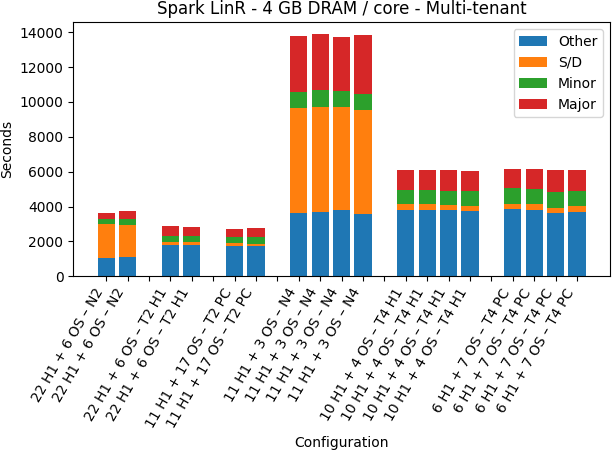
\includegraphics[width=\linewidth]{./fig/linr64.png}
    \caption{Execution time breakdown for multiple instances of
    LinearRegression using the 64 GB total DRAM setup. E.g.
    22-28-64-Native 1 indicates the first of the 2-4-8 instances that
    was run in parallel and uses 22 GB H1 - 28 GB total cgroup DRAM
    and 64 GB total DRAM for the machine.}
    \label{fig:linr64}
\end{subfigure}
\begin{subfigure}[b]{0.48\textwidth}
    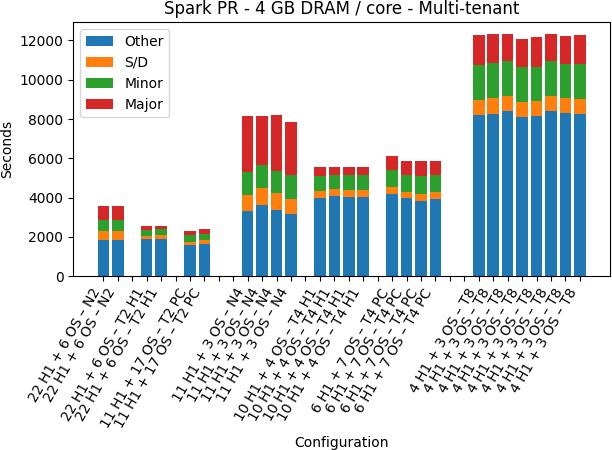
\includegraphics[width=\linewidth]{./fig/pr64.png}
    \caption{Execution time breakdown for multiple instances of
    PageRank using the 64 GB total DRAM setup. E.g. 22-28-64-Native 1
    indicates the first of the 2-4-8 instances that was run in
    parallel and uses 22 GB H1 - 28 GB total cgroup DRAM and 64 GB
    total DRAM for the machine.}
    \label{fig:pr64}
\end{subfigure}\\[1em]
\end{figure}

\begin{figure}[htbp]
	\centering
        \begin{subfigure}[b]{0.48\textwidth}
    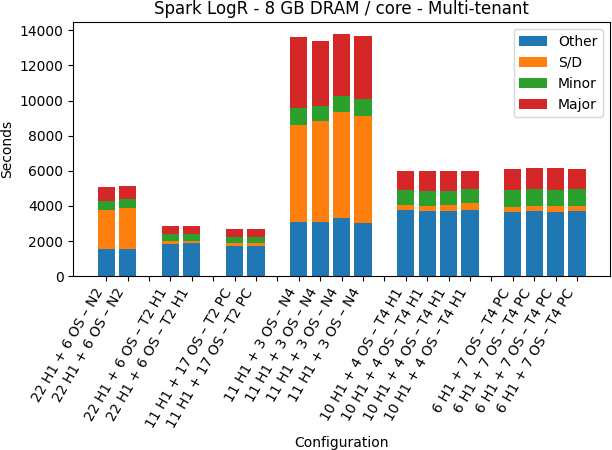
\includegraphics[width=\linewidth]{./fig/logr64.png}
    \caption{Execution time breakdown for multiple instances of
    Logistic Regression using the 64 GB total DRAM setup. E.g.
    22-28-64-Native 1 indicates the first of the 2-4-8 instances that
    was run in parallel and uses 22 GB H1 - 28 GB total cgroup DRAM
    and 64 GB total DRAM for the machine.}
    \label{fig:logr64}
\end{subfigure}

\begin{subfigure}[b]{0.48\textwidth}
    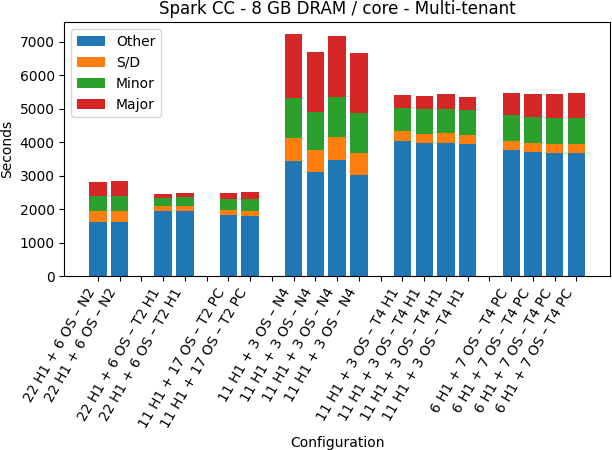
\includegraphics[width=\linewidth]{./fig/cc64.png}
    \caption{Execution time breakdown for multiple instances of
    Connected Component using the 64 GB total DRAM setup. E.g.
    22-28-64-Native 1 indicates the first of the 2-4-8 instances that
    was run in parallel and uses 22 GB H1 - 28 GB total cgroup DRAM
    and 64 GB total DRAM for the machine.}
    \label{fig:cc64}
\end{subfigure}\\[1em]
\end{figure}

\begin{figure}[htbp]
	\centering
	\begin{subfigure}[b]{0.48\textwidth}
    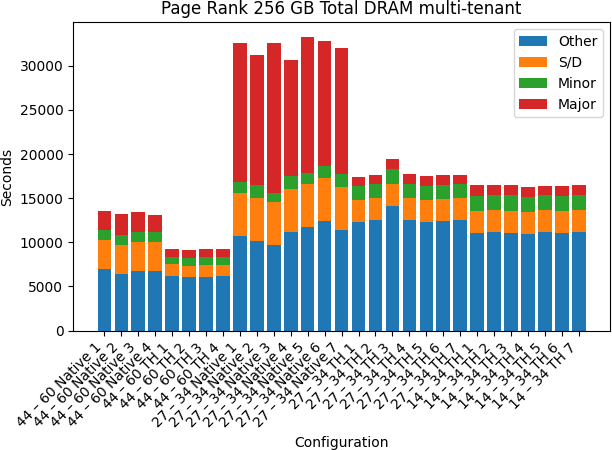
\includegraphics[width=\linewidth]{./fig/pr256.png}
    \caption{Execution time breakdown for multiple instances of
    PageRank using the 256 GB total DRAM setup. E.g. 44-60-256-Native
    1 indicates the first of the 2-4-8 instances that was run in
    parallel and uses 44 GB H1 - 60 GB total cgroup DRAM and 256 GB
    total DRAM for the machine.} 
    \label{fig:pr256}
	\end{subfigure}
\begin{subfigure}[b]{0.48\textwidth}
    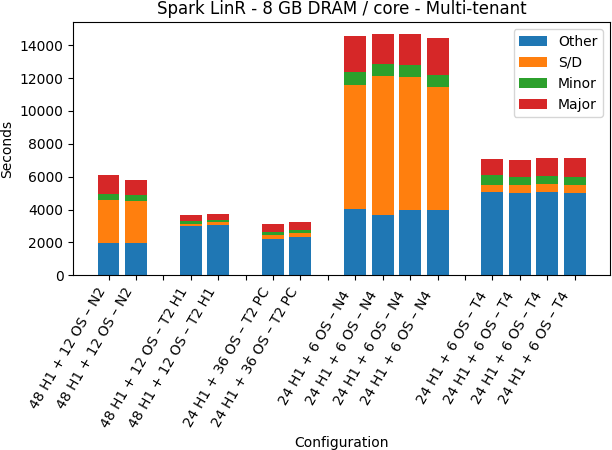
\includegraphics[width=\linewidth]{./fig/linr128.png}
    \caption{Execution time breakdown for multiple instances of
    LinearRegression using the 128 GB total DRAM setup. E.g.
    22-28-64-Native 1 indicates the first of the 2-4-8 instances that
    was run in parallel and uses 22 GB H1 - 28 GB total cgroup DRAM
    and 64 GB total DRAM for the machine.}
    \label{fig:linr128}
\end{subfigure}
\end{figure}


\subsection{Experiments with colocated instances}

Here we look at the colocated experiments of Spark and Giraph.
We explain each figure from 2 aspects:
\begin{itemize}
\item{The differences in the time breakdown while number of instances increase for each configuration.}
\item{A comparison between the different configurations while instances increase.}
\end{itemize}

Figure \ref{fig:linr64} shows the performance of multiple
Native-TeraHeap Spark instances running LinearRegression with 64 GB
dataset per instance in our 64 GB DRAM machine. Each instance of Spark
uses one executor with 8 cores per executor. Available DRAM is 56 GB
and 8 GB are left to the Operating system, resulting in 64 GB total
DRAM. All configurations utilize 56 of 64 GB total DRAM. 
Starting from the left of the graph, the first 6 bars show the
performance of 3 runs. The first run is with 2 colocated Native Spark instances.
Another run with 2 colocated TH Spark instances with H1 dominating Page Cache
and a third run with 2 colocated TH Spark instances where Page Cache dominates H1. 
Each instance of the first 2 runs uses 22 GB DRAM for H1 (Java Heap) and 6 GB for rest of the services.
The third run uses 11 GB DRAM for H1 and 17 GB for Page Cache for each instance. 
The rest 12 bars show the performance of another 3 runs. The first run is with 4 colocated Native Spark instances.
Another run with 4 colocated TH Spark instances with H1 dominating Page Cache
and a third run with 4 colocated TH Spark instances where Page Cache dominates H1. 
Each instance of the first run uses 11 GB DRAM for H1 (Java Heap) and 3 GB for rest of the services. 
The second run uses 10 GB DRAM for H1 and 4 GB for Page Cache for each instance. 
The third run uses 6 GB DRAM for H1 and 8 GB for Page Cache for each instance. 
Considering the first aspect we see that GC and S/D increase dramatically for Native Spark along with significant increase to Other time. GC differences are witnessed because the heap capacity decreases and that causes memory pressure. TeraHeap Spark shows a slight increase to Major GC while the number of instances increases. This is because of the decreased heap capacity. Other time increases because more objects are moved to TeraHeap and read/write traffic increases but this is a good trade-off because all the GC is absorbed. S/D is completely absorbed by MMIO. From the third aspect, as instances increase in the server the benefit gap between Native and TeraHeap Spark becomes bigger. As Native Spark starves from more GC and S/D, TeraHeap maintains its benefits. 

Figure \ref{fig:pr64} shows the performance of multiple
Native-TeraHeap Spark instances running PageRank with 8 GB
dataset per instance in our 64 GB DRAM machine. Each instance of Spark
uses one executor with 8 cores per executor. Available DRAM is 56 GB
and 8 GB are left to the Operating system, resulting in 64 GB total
DRAM. All configurations utilize 56 of 64 GB total DRAM.
Starting from the left of the graph, the first 6 bars show the
performance of 3 runs. The first run is with 2 colocated Native Spark instances.
Another run with 2 colocated TH Spark instances with H1 dominating Page Cache
and a third run with 2 colocated TH Spark instances where Page Cache dominates H1.
Each instance of the first 2 runs uses 22 GB DRAM for H1 (Java Heap) and 6 GB for rest of the services.
The third run uses 11 GB DRAM for H1 and 17 GB for Page Cache for each instance. 
The next 12 bars show the performance of another 3 runs. The first run is with 4 colocated Native Spark instances.
Another run with 4 colocated TH Spark instances with H1 dominating Page Cache
and a third run with 4 colocated TH Spark instances where Page Cache dominates H1.
Each instance of the first run uses 11 GB DRAM for H1 (Java Heap) and 3 GB for rest of the services.
The second run uses 10 GB DRAM for H1 and 4 GB for Page Cache for each instance.
The third run uses 6 GB DRAM for H1 and 8 GB for Page Cache for each instance.
The last 8 bars refer to 8 colocated instances of TeraHeap Spark only. 
We were unable to decrease H1 enough to run 8 colocates instance of Native Spark
because JVM runs out of memory. Each instance of the run uses 4 GB DRAM for H1 (Java Heap) and 3 GB for Page Cache.
Considering the first aspect we see that Minor and Major GC increase dramatically for Native Spark along with significant increase to Other time. Minor and Major GC differences are witnessed because the heap capacity decreases and that causes memory pressure. TeraHeap Spark shows a slight increase to Major GC while the number of instances increases. This is because of the decreasing heap capacity. Other time increases because more objects are moved to TeraHeap but this is a good trade-off because all the GC is absorbed. S/D is completely absorbed by MMIO. From the second aspect, as instances increase in the server the benefit gap between Native and TeraHeap Spark becomes bigger. As Native Spark starves from more GC and S/D, TeraHeap maintains its benefits.

Figure \ref{fig:logr64} shows the performance of multiple
Native-TeraHeap Spark instances running Logistic Regression with 64 GB
dataset per instance in our 64 GB DRAM machine. Each instance of Spark
uses one executor with 8 cores per executor. Available DRAM is 56 GB
and 8 GB are left to the Operating system, resulting in 64 GB total
DRAM. All configurations utilize 56 of 64 GB total DRAM.
Starting from the left of the graph, the first 6 bars show the
performance of 3 runs. The first run is with 2 colocated Native Spark instances.
Another run with 2 colocated TH Spark instances with H1 dominating Page Cache
and a third run with 2 colocated TH Spark instances where Page Cache dominates H1.
Each instance of the first 2 runs uses 22 GB DRAM for H1 (Java Heap) and 6 GB for rest of the services.
The third run uses 11 GB DRAM for H1 and 17 GB for Page Cache for each instance. 
The next 12 bars show the performance of another 3 runs. The first run is with 4 colocated Native Spark instances.
Another run with 4 colocated TH Spark instances with H1 dominating Page Cache
and a third run with 4 colocated TH Spark instances where Page Cache dominates H1.
Each instance of the first run uses 11 GB DRAM for H1 (Java Heap) and 3 GB for rest of the services.
The second run uses 10 GB DRAM for H1 and 4 GB for Page Cache for each instance.
The third run uses 6 GB DRAM for H1 and 8 GB for Page Cache for each instance.
Considering the first aspect we see that GC and S/D increase dramatically for Native Spark along with significant increase to Other time. GC differences are witnessed because the heap capacity decreases and that causes memory pressure. TeraHeap Spark shows a slight increase to Major GC while the number of instances increases. This is because of the decreased heap capacity. Other time increases because more objects are moved to TeraHeap and read/write traffic increases but this is a good trade-off because all the GC is absorbed. S/D is completely absorbed by MMIO. From the third aspect, as instances increase in the server the benefit gap between Native and TeraHeap Spark becomes bigger. As Native Spark starves from more GC and S/D, TeraHeap maintains its benefits. 

Figure \ref{fig:cc64} shows the performance of multiple
Native-TeraHeap Spark instances running Connected Component with 8 GB
dataset per instance in our 64 GB DRAM machine. Each instance of Spark
uses one executor with 8 cores per executor. Available DRAM is 56 GB
and 8 GB are left to the Operating system, resulting in 64 GB total
DRAM. All configurations utilize 56 of 64 GB total DRAM.
Starting from the left of the graph, the first 6 bars show the
performance of 3 runs. The first run is with 2 colocated Native Spark instances.
Another run with 2 colocated TH Spark instances with H1 dominating Page Cache
and a third run with 2 colocated TH Spark instances where Page Cache dominates H1.
Each instance of the first 2 runs uses 22 GB DRAM for H1 (Java Heap) and 6 GB for rest of the services.
The third run uses 11 GB DRAM for H1 and 17 GB for Page Cache for each instance. 
The next 12 bars show the performance of another 3 runs. The first run is with 4 colocated Native Spark instances.
Another run with 4 colocated TH Spark instances with H1 dominating Page Cache
and a third run with 4 colocated TH Spark instances where Page Cache dominates H1.
Each instance of the first run uses 11 GB DRAM for H1 (Java Heap) and 3 GB for rest of the services.
The second run uses 10 GB DRAM for H1 and 4 GB for Page Cache for each instance.
The third run uses 6 GB DRAM for H1 and 8 GB for Page Cache for each instance.
Considering the first aspect we see that Minor and Major GC increase dramatically for Native Spark along with significant increase to Other time. Minor and Major GC differences are witnessed because the heap capacity decreases and that causes memory pressure. TeraHeap Spark shows a slight increase to Major GC while the number of instances increases. This is because of the decreasing heap capacity. Other time increases because more objects are moved to TeraHeap but this is a good trade-off because all the GC is absorbed. S/D is completely absorbed by MMIO. From the second aspect, as instances increase in the server the benefit gap between Native and TeraHeap Spark becomes bigger. As Native Spark starves from more GC and S/D, TeraHeap maintains its benefits.

Figure \ref{fig:pr256} shows the performance of multiple
Native-TeraHeap Spark instances running PageRank with 32 GB
dataset per instance in our 256 GB DRAM machine. Each instance of Spark
uses one executor with 8 cores per executor. Available DRAM is 240 GB
and 16 GB are left to the Operating system, resulting in 256 GB total
DRAM. All configurations utilize 240 of 256 GB total DRAM.
Starting from the left of the graph, the first 8 bars show the
performance of 2 runs. The first run is with 4 colocated Native Spark instances.
Another run with 4 colocated TH Spark instances with H1 dominating Page Cache.
Each instance of the first 8 runs uses 48 GB DRAM for H1 (Java Heap) and 12 GB for rest of the services including Page Cache.
The next 21 bars show the performance of another 3 runs. The first run is with 7 colocated Native Spark instances.
Another run with 7 colocated TH Spark instances with H1 dominating Page Cache
and a third run with 7 colocated TH Spark instances where Page Cache dominates H1.
Each instance of the first run uses 27 GB DRAM for H1 (Java Heap) and 7 GB for rest of the services.
The second run uses 27 GB DRAM for H1 and 7 GB for Page Cache for each TH instance.
The third run uses 14 GB DRAM for H1 and 20 GB for Page Cache for each TH instance.
Considering the first aspect we see that Minor and Major GC increase dramatically for Native Spark along with significant increase to Other time. Minor and Major GC differences are witnessed because the heap capacity decreases and that causes memory pressure. TeraHeap Spark shows a slight increase to Major GC while the number of instances increases. This is because of the decreasing heap capacity. Other time increases because more objects are moved to TeraHeap but this is a good trade-off because all the GC is absorbed. S/D is completely absorbed by MMIO. From the second aspect, as instances increase in the server the benefit gap between Native and TeraHeap Spark becomes bigger. As Native Spark starves from more GC and S/D, TeraHeap maintains its benefits.

\subsection{Is the CPU utilization of the server increasing
accordingly to throughput?}
\begin{figure}[htbp]
	\centering
	\begin{subfigure}[b]{0.48\textwidth}
        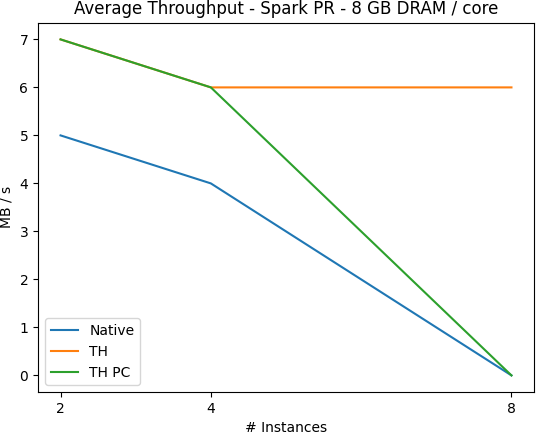
\includegraphics[width=\linewidth]{./fig/PR_64_THR.png}
    \caption{Page Rank 64 GB DRAM setup Native and TeraHeap throughput
    as the number of instances increases. Configurations starting with
    N denote a run with Native instances of Spark and with T with
    TeraHeap. H1 is a run with the memory budget configured to contain
    a bigger size for H1 than PageCache and PC the opposite. E.g. T2
    PC is a run of 2 concurrent TeraHeap instances with exactly the
    same configuration.}
\label{fig:pr_64_thr}
\end{subfigure}
        \begin{subfigure}[b]{0.48\textwidth}
        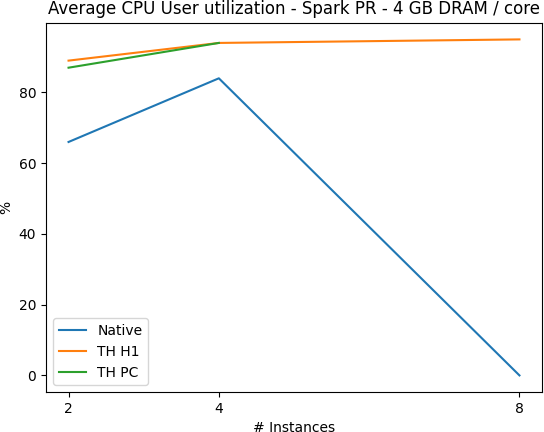
\includegraphics[width=\linewidth]{./fig/PR_64_USR.png}
    \caption{Page Rank 64 GB DRAM setup Native and TeraHeap User CPU utilization
    as the number of instances increases. Configurations starting with
    N denote a run with Native instances of Spark and with T with
    TeraHeap. H1 is a run with the memory budget configured to contain
    a bigger size for H1 than PageCache and PC the opposite. E.g. T2
    PC is a run of 2 concurrent TeraHeap instances with exactly the
    same configuration.}
		\label{fig:pr_64_usr}
	\end{subfigure}\\[1em]
\end{figure}

\begin{figure}[htbp]
	\centering
        \begin{subfigure}[b]{0.48\textwidth}
        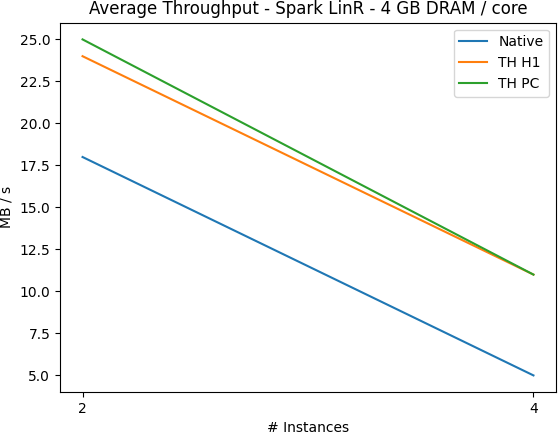
\includegraphics[width=\linewidth]{./fig/LINR_64_THR.png}
    \caption{Linear Regression 64 GB DRAM setup Native and TeraHeap
    throughput as the number of instances increases. Configurations
    starting with N denote a run with Native instances of Spark and
    with T with TeraHeap. H1 is a run with the memory budget
    configured to contain a bigger size for H1 than PageCache and PC
    the opposite. E.g. T2 PC is a run of 2 concurrent TeraHeap
    instances with exactly the same configuration.}
		\label{fig:linr_64_thr}
        \end{subfigure}
        \begin{subfigure}[b]{0.48\textwidth}
        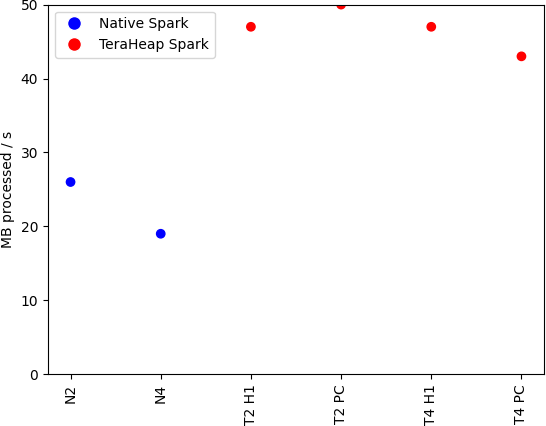
\includegraphics[width=\linewidth]{./fig/LOGR_64_THR.png}
    \caption{Logistic Regression 64 GB DRAM setup Native and TeraHeap
    throughput as the number of instances increases. Configurations
    starting with N denote a run with Native instances of Spark and
    with T with TeraHeap. H1 is a run with the memory budget
    configured to contain a bigger size for H1 than PageCache and PC
    the opposite. E.g. T2 PC is a run of 2 concurrent TeraHeap
    instances with exactly the same configuration.}
		\label{fig:logr_64_thr}
        \end{subfigure}\\[1em]
\end{figure}

\begin{figure}[htbp]
	\centering
        \begin{subfigure}[b]{0.48\textwidth}
        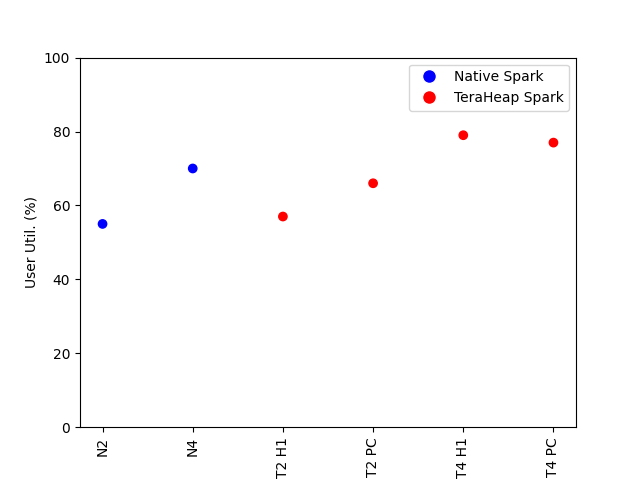
\includegraphics[width=\linewidth]{./fig/LINR_64_USR.png}
    \caption{Linear Regression 64 GB DRAM setup Native and TeraHeap
    User CPU utilization as the number of instances increases. Configurations
    starting with N denote a run with Native instances of Spark and
    with T with TeraHeap. H1 is a run with the memory budget
    configured to contain a bigger size for H1 than PageCache and PC
    the opposite. E.g. T2 PC is a run of 2 concurrent TeraHeap
    instances with exactly the same configuration.}
		\label{fig:linr_64_usr}
        \end{subfigure}
   \begin{subfigure}[b]{0.48\textwidth}
    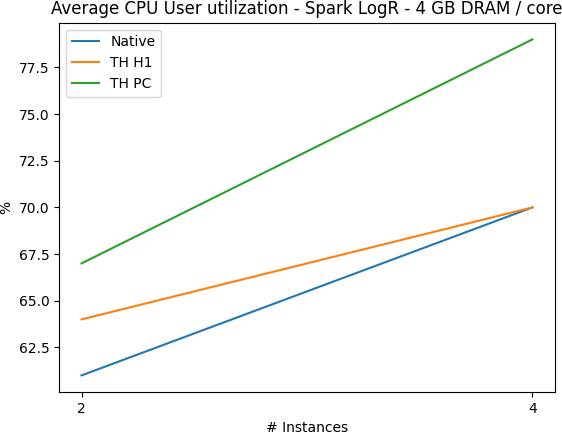
\includegraphics[width=\linewidth]{./fig/LOGR_64_USR.png}
    \caption{Logistic Regression 64 GB DRAM setup Native and TeraHeap
    User CPU utilization as the number of instances increases. Configurations
    starting with N denote a run with Native instances of Spark and
    with T with TeraHeap. H1 is a run with the memory budget
    configured to contain a bigger size for H1 than PageCache and PC
    the opposite. E.g. T2 PC is a run of 2 concurrent TeraHeap
    instances with exactly the same configuration.}
	   \label{fig:logr_64_usr}
    \end{subfigure}\\[1em]
\end{figure}

\begin{figure}[htbp]
	\centering
        \begin{subfigure}[b]{0.48\textwidth}
        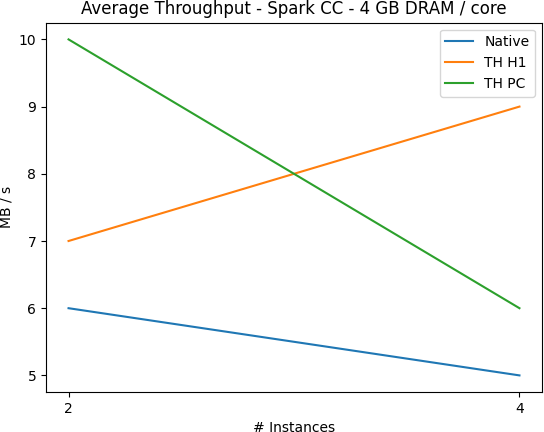
\includegraphics[width=\linewidth]{./fig/CC_64_THR.png}
    \caption{Connected Component 64 GB DRAM setup Native and TeraHeap
    throughput as the number of instances increases.Configurations
    starting with N denote a run with Native instances of Spark and
    with T with TeraHeap. H1 is a run with the memory budget
    configured to contain a bigger size for H1 than PageCache and PC
    the opposite. E.g. T2 PC is a run of 2 concurrent TeraHeap
    instances with exactly the same configuration. }
		\label{fig:cc_64_thr}
	\end{subfigure}
\begin{subfigure}[b]{0.48\textwidth}
        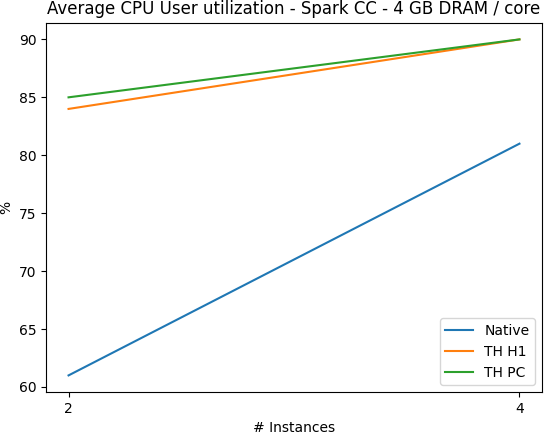
\includegraphics[width=\linewidth]{./fig/CC_64_USR.png}
    \caption{Connected Component 64 GB DRAM setup Native and TeraHeap
    User CPU utilization as the number of instances increases. Configurations
    starting with N denote a run with Native instances of Spark and
    with T with TeraHeap. H1 is a run with the memory budget
    configured to contain a bigger size for H1 than PageCache and PC
    the opposite. E.g. T2 PC is a run of 2 concurrent TeraHeap
    instances with exactly the same configuration.}
	\label{fig:cc_64_usr}
\end{subfigure}\\[1em]
\end{figure}

\begin{figure}[htbp]
        \centering
        \begin{subfigure}[b]{0.48\textwidth}
        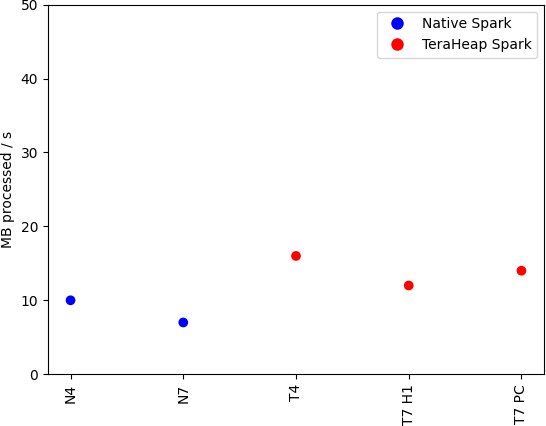
\includegraphics[width=\linewidth]{./fig/PR_256_THR.png}
    \caption{Page Rank 256 GB DRAM setup Native and TeraHeap
    throughput as the number of instances increases.Configurations
    starting with N denote a run with Native instances of Spark and
    with T with TeraHeap. H1 is a run with the memory budget
    configured to contain a bigger size for H1 than PageCache and PC
    the opposite. E.g. T2 PC is a run of 2 concurrent TeraHeap
    instances with exactly the same configuration. }
                \label{fig:pr_256_thr}
        \end{subfigure}
\begin{subfigure}[b]{0.48\textwidth}
        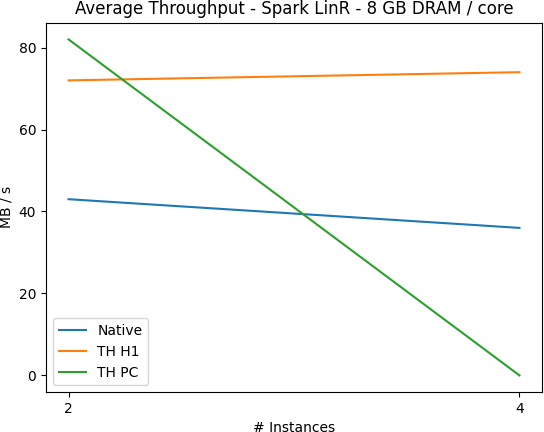
\includegraphics[width=\linewidth]{./fig/LINR_128_THR.png}
    \caption{Linear Regression 128 GB DRAM setup Native and TeraHeap
    throughput as the number of instances increases. Configurations
    starting with N denote a run with Native instances of Spark and
    with T with TeraHeap. H1 is a run with the memory budget
    configured to contain a bigger size for H1 than PageCache and PC
    the opposite. E.g. T2 PC is a run of 2 concurrent TeraHeap
    instances with exactly the same configuration.}
        \label{fig:linr_128_thr}
\end{subfigure}\\[1em]
\end{figure}

\begin{figure}[htbp]
        \centering
        \begin{subfigure}[b]{0.48\textwidth}
        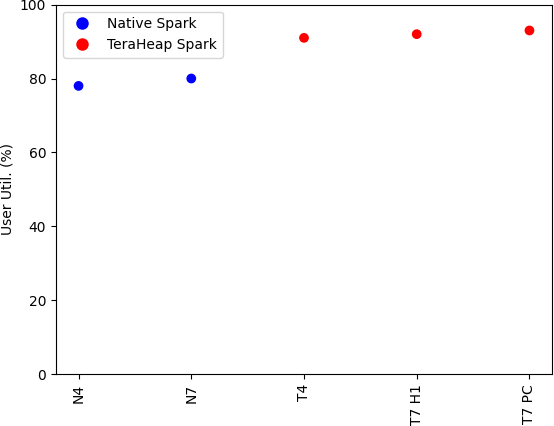
\includegraphics[width=\linewidth]{./fig/PR_256_USR.png}
    \caption{Page Rank 256 GB DRAM setup Native and TeraHeap
    User CPU utilization as the number of instances increases.Configurations
    starting with N denote a run with Native instances of Spark and
    with T with TeraHeap. H1 is a run with the memory budget
    configured to contain a bigger size for H1 than PageCache and PC
    the opposite. E.g. T2 PC is a run of 2 concurrent TeraHeap
    instances with exactly the same configuration. }
                \label{fig:pr_256_usr}
        \end{subfigure}
\begin{subfigure}[b]{0.48\textwidth}
        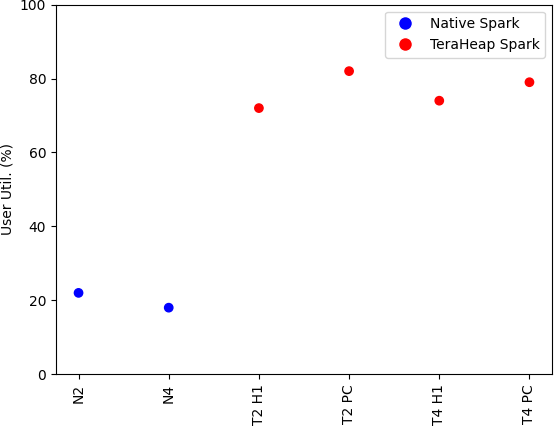
\includegraphics[width=\linewidth]{./fig/LINR_128_USR.png}
    \caption{Linear Regression 128 GB DRAM setup Native and TeraHeap
    User CPU utilization as the number of instances increases. Configurations
    starting with N denote a run with Native instances of Spark and
    with T with TeraHeap. H1 is a run with the memory budget
    configured to contain a bigger size for H1 than PageCache and PC
    the opposite. E.g. T2 PC is a run of 2 concurrent TeraHeap
    instances with exactly the same configuration.}
        \label{fig:linr_128_usr}
\end{subfigure}\\[1em]
\end{figure}


The main goal for colocating tasks is to increase the CPU utilization and achieve better
throughput. CPU utilization is split to 2 parts. 
User utilization includes all CPU cycles that were executed in user-space threads.
It includes GC cycles, S/D cycles and mutator tasks except I/O.
System utilization includes all CPU cycles that were executed in kernel-space threads.
This includes I/O carried out by GC (TeraHeap) and mutator I/O.
Therefore we have to focus to User utilization which includes the effective CPU cycles done by the application.
By looking at figures \ref{fig:pr_64_thr}, \ref{fig:linr_64_thr},
\ref{fig:logr_64_thr} and \ref{fig:cc_64_thr} we see that Native
Spark's throughput decreases as the number of colocated
instances-executors increase in the server.
This is justified by GC and S/D that increase as instances increase and by the increased User utilization
(\ref{fig:pr_64_usr}, \ref{fig:linr_64_usr}, \ref{fig:logr_64_usr}, \ref{fig:cc_64_usr}).
TeraHeap achieves higher throughput than Native Spark and that is also justified by the increased User utilization.
Having higher user utilization and lower GC and S/D means that effective CPU utilization is really higher, since more
work is done by mutator threads.

\subsection{Single instance vs colocated instances}
When running colocated instances the goal is that the execution 
of all instances is close to the summary of execution of all instances run isolated.
As seen in tables, most of the times we are not even close. To achieve that
we need a scheduling policy to dynamically resize H1 and Page Cache based on runtime decisions.

\subsection{What
happens with monetary cost across different cloud platforms?}

\iffalse
\begin{table}[htbp]
  \centering
	\begin{subtable}[b]{0.45\linewidth}
  \caption{Page Rank synopsis table. Configurations starting
    with N denote a run with Native instances of Spark and with T with
    TeraHeap. H1 is a run with the memory budget configured to contain
    a bigger size for H1 than PageCache and PC the opposite.}
  \label{tab:pr_table}
        %\resizebox{19cm}{!}{
        \begin{tabular}{|c|c|c|c|c|c|c|c|c|c|c|c|c|}
      \hline
\textbf{Conf.} & \textbf{H1 Size/I} & \textbf{Memory/I} & \textbf{Total Mem.} & \textbf{\#I} & \textbf{Exec. Time} & \textbf{CPU Idle} & \textbf{Total MB Proc.} & \textbf{MB/s} & \textbf{MB/s/I} & \textbf{Cost AWS \$} & \textbf{Cost GCP \$} & \textbf{Cost Azure \$} \\
        \hline
    N2 - small & 22 & 28 & 64 & 2 & 3563 & 29 & 16980 & 5 & 2 & 0.6 & 0.58 & 0.67 \\
    N4 - small & 11 & 14 & 64 & 4 & 8195 & 11 & 33960 & 4 & 1 & 1.8 & 1.74 & 2.01 \\
    T2 H1 – small & 22 & 28 & 64 & 2 & 2545 & 7 & 16980 & 7 & 3 & 0.6 & 0.58 & 0.67 \\
    T2 PC – small & 11 & 28 & 64 & 2 & 2385 & 9 & 16980 & 7 & 4 & 0.6 & 0.58 & 0.67 \\
    T4 H1 – small & 11 & 14 & 64 & 4 & 5554 & 1 & 33960 & 6 & 2 & 1.2 & 1.16 & 1.34 \\
    T4 PC – small & 6 & 14 & 64 & 4 & 5880 & 1 & 33960 & 6 & 2 & 1.2 & 1.16 & 1.34 \\
    N8 – small & 4 & 7 & 64 & 8 & OOM & ** & 0 & 0 & 0 & *** & *** & *** \\
    T8 – small & 4 & 7 & 64 & 8 & 12305 & 0 & 67920 & 6 & 1 & 2.4 & 2.32 & 2.68 \\
    N4 - big & 44 & 60 & 256 & 4 & 13542 & 15 & 135872 & 10 & 3 & 6.4 & *** & *** \\
    T4 – big & 48 & 60 & 256 & 4 & 9284 & 5 & 135782 & 16 & 4 \\      
	\hline
     \end{tabular}%
        %}
\end{subtable}

	\begin{subtable}[b]{0.45\linewidth}
  \caption{Linear Regression synopsis table. Configurations starting
    with N denote a run with Native instances of Spark and with T with
    TeraHeap. H1 is a run with the memory budget configured to contain
    a bigger size for H1 than PageCache and PC the opposite.}
  \label{tab:linr_table}
        %\resizebox{19cm}{!}{
        \begin{tabular}{|c|c|c|c|c|c|c|c|c|c|c|c|c|}
      \hline
\textbf{Conf.} & \textbf{H1 Size/I} & \textbf{Memory/I} & \textbf{Total Mem.} & \textbf{\#I} & \textbf{Exec. Time} & \textbf{CPU Idle} & \textbf{Total MB Proc.} & \textbf{MB/s} & \textbf{MB/s/I} & \textbf{Cost AWS \$} & \textbf{Cost GCP \$} & \textbf{Cost Azure \$} \\
	\hline 
      N2 & 22 & 28 & 64 & 2 & 3745 & 20 & 134896 & 37 & 18 & 0.6 & 0.58 & 0.67 \\ 
      N4 & 11 & 14 & 64 & 4 & 13874 & 7 & 269792 & 20 & 5 & 2.4 & 2.32 & 2.01 \\
      T2 H1 & 22 & 28 & 64 & 2 & 2891 & 19 & 134896 & 48 & 24 & 0.6 & 0.58 & 0.67 \\
      T2 PC & 11 & 28 & 64 & 2 & 2747 & 18 & 134896 & 49 & 25 & 0.6 & 0.58 & 0.67 \\
      T4 H1 & 11 & 14 & 64 & 4 & 6075 & 2 & 269792 & 44 & 11 & 1.2 & 1.16 & 1.34 \\
      T4 PC & 6 & 14 & 64 & 4 & 6176 & 3 & 269792 & 44 & 11 & 1.2 & 1.16 & 1.34 \\ 
      \hline
     \end{tabular}%
	%}
\end{subtable}
	\vspace{1em}
\end{table}
\fi
\iffalse
%\begin{center}%[htbp]
 %   \centering
  %  \caption{Page Rank synopsis table}
	%\begin{tabular}{|c|c|c|c|c|c|c|c|c|c|c|c|c|c|c|c|c|}
		\begin{tabularx}{\linewidth}{*{17}{X}}
	    \hline
        Configuration & H1 Size / I & Memory / I & Total memory & \#I & Exec. Time & User util. & System util. & IO Wait & CPU Idle & Total MB Processed & MB/s & MB/s/I & Cost AWS \$ & Cost GCP \$ & Cost Azure \$ \\
        \hline
        N2-small – single & 22 & 28 & 64 & 1 & 1762 & 32 & 2 & 1 & 65 & 8490 & 5 & 5 & 0.6 & 0.58 & 0.67 \\
        N2 - small & 22 & 28 & 64 & 2 & 3563 & 66 & 5 & 2 & 27 & 16980 & 5 & 2 & 0.6 & 0.58 & 0.67 \\
        N4 – small – single & 11 & 14 & 64 & 1 & 1783 & 29 & 2 & 1 & 68 & 8490 & 5 & 5 & 0.6 & 0.58 & 0.67 \\
        N4 - small & 11 & 14 & 64 & 4 & 8195 & 84 & 6 & 2 & 8 & 33960 & 4 & 1 & 1.8 & 1.74 & 2.01 \\
        N8 – small & 4 & 7 & 64 & 8 & OOM & 0 & 0 & 0 & ** & 0 & 0 & 0 & *** & *** \\
        T2 H1- small – single & 22 & 28 & 64 & 1 & 1146 & 46 & 2 & 1 & 51 & 8490 & 7 & 7 & 0.6 & 0.58 & 0.67 \\
        T2 H1 – small & 22 & 28 & 64 & 2 & 2545 & 89 & 4 & 1 & 6 & 16980 & 7 & 3 & 0.6 & 0.58 & 0.67 \\
        T2 PC- small – single & 11 & 28 & 64 & 1 & 966 & 45 & 2 & 1 & 52 & 8490 & 9 & 9 & 0.6 & 0.58 & 0.67 \\
        T2 PC – small & 11 & 28 & 64 & 2 & 2385 & 87 & 4 & 0 & 9 & 16980 & 7 & 4 & 0.6 & 0.58 & 0.67 \\
        T4 H1 – small – single & 11 & 14 & 64 & 1 & 984 & 43 & 3 & 1 & 53 & 8490 & 9 & 9 & 0.6 & 0.58 & 0.67 \\
        T4 H1 – small & 11 & 14 & 64 & 4 & 5554 & 94 & 5 & 0 & 1 & 33960 & 6 & 2 & 1.2 & 1.16 & 1.34 \\
        T4 PC – small – single & 6 & 14 & 64 & 1 & 922 & 42 & 2 & 2 & 54 & 8490 & 9 & 9 & 0.6 & 0.58 & 0.67 \\
        T4 PC – small & 6 & 14 & 64 & 4 & 5880 & 94 & 5 & 0 & 1 & 33960 & 6 & 2 & 1.2 & 1.16 & 1.34 \\
        T8 – small – single & 4 & 7 & 64 & 1 & 1037 & 39 & 2 & 1 & 58 & 8490 & 8 & 8 & 0.6 & 0.58 & 0.67 \\
        T8 – small & 4 & 7 & 64 & 8 & 12305 & 95 & 5 & 0 & 0 & 67920 & 6 & 1 & 2.4 & 2.32 & 2.68 \\
        N4 - big & 48 & 60 & 256 & 4 & 13542 & 78 & 7 & 7 & 8 & 135872 & 10 & 3 & 6.4 & *** & *** \\
        T4 – big & 48 & 60 & 256 & 4 & 9284 & 91 & 8 & 1 & 1 & 135782 & 16 & 4 & 1.8 & *** & *** \\
        N7 – big & 27 & 34 & 256 & 7 & 32763 & 80 & 8 & 12 & 0 & 237776 & 7 & 1 & 14.4 & *** & *** \\
        T7 H1 – big & 27 & 34 & 256 & 7 & 19443 & 92 & 7 & 1 & 0 & 237776 & 12 & 2 & 9.6 & *** & *** \\
        T7 PC – big & 14 & 34 & 256 & 7 & 16485 & 93 & 7 & 1 & 0 & 237776 & 14 & 2 & 8 & *** & *** \\
        \hline
	\bottomrule
    \end{tabularx}
%	\label{tab:pr_table}
%\end{center}
\fi
\iffalse
\begin{table}[t!]
  \centering
  \caption{Logistic Regression synopsis table. Configurations starting
    with N denote a run with Native instances of Spark and with T with
    TeraHeap. H1 is a run with the memory budget configured to contain
    a bigger size for H1 than PageCache and PC the opposite.}
  \label{tab:logr_table}
	\resizebox{19cm}{!}{
	\begin{tabular}{|c|c|c|c|c|c|c|c|c|c|c|c|c|}
      \hline
\textbf{Conf.} & \textbf{H1 Size/I} & \textbf{Memory/I} & \textbf{Total Mem.} & \textbf{\#I} & \textbf{Exec. Time} & \textbf{CPU Idle} & \textbf{Total MB Proc.} & \textbf{MB/s} & \textbf{MB/s/I} & \textbf{Cost AWS \$} & \textbf{Cost GCP \$} & \textbf{Cost Azure \$} \\
      \hline
      N2 & 22 & 28 & 64 & 2 & 5127 & 18 & 133348 & 26 & 13 & 1.2 & 1.16 & 0.67 \\
      N4 & 11 & 14 & 64 & 4 & 13730 & 7 & 266696 & 19 & 5 & 2.4 & 2.32 & 2.68 \\
      T2 H1 & 22 & 28 & 64 & 2 & 2861 & 18 & 133348 & 47 & 24 & 0.6 & 0.58 & 0.67 \\
      T2 PC & 11 & 28 & 64 & 2 & 2683 & 18 & 133348 & 50 & 25 & 0.6 & 0.58 & 0.67 \\
      T4 H1 & 10 & 14 & 64 & 4 & 5712 & 2 & 266696 & 47 & 12 & 1.2 & 1.16 & 1.34 \\
      T4 PC & 6 & 14 & 64 & 4 & 6138 & 2 & 266696 & 43 & 10 & 1.2 & 1.16 & 1.34 \\
      \hline
     \end{tabular}%
	}
\end{table}

\begin{table}[t!]
  \centering
  \caption{Connected Component synopsis table. Configurations starting
    with N denote a run with Native instances of Spark and with T with
    TeraHeap. H1 is a run with the memory budget configured to contain
    a bigger size for H1 than PageCache and PC the opposite.}
  \label{tab:cc_table}
        \resizebox{19cm}{!}{
        \begin{tabular}{|c|c|c|c|c|c|c|c|c|c|c|c|c|}
      \hline
\textbf{Conf.} & \textbf{H1 Size/I} & \textbf{Memory/I} & \textbf{Total Mem.} & \textbf{\#I} & \textbf{Exec. Time} & \textbf{CPU Idle} & \textbf{Total MB Proc.} & \textbf{MB/s} & \textbf{MB/s/I} & \textbf{Cost AWS \$} & \textbf{Cost GCP \$} & \textbf{Cost Azure \$} \\
	\hline
      N2 & 22 & 28 & 64 & 2 & 2958 & 26 & 16980 & 6 & 3 & 0.6 & 0.58 & 0.67 \\
      N4 & 11 & 14 & 64 & 4 & 7231 & 7 & 33960 & 5 & 3 & 1.8 & 1.74 & 2.01 \\
      T2 H1 & 22 & 28 & 64 & 2 & 2526 & 5 & 16980 & 7 & 4 & 0.6 & 0.58 & 0.67 \\
      T2 PC & 11 & 28 & 64 & 2 & 2519 & 7 & 16980 & 7 & 4 & 0.6 & 0.58 & 0.67 \\
      T4 H1 & 11 & 14 & 64 & 4 & 5439 & 3 & 33960 & 6 & 3 & 1.2 & 0.58 & 0.67 \\
      T4 PC & 6 & 14 & 64 & 4 & 5487 & 2 & 33960 & 6 & 3 & 1.2 & 1.16 & 1.34 \\
      \hline
     \end{tabular}%
	}
\end{table}
\fi

Tables \ref{tab:pr_table}, \ref{tab:linr_table}, \ref{tab:logr_table}
and \ref{tab:cc_table} show 
Amazon Web Services Cloud (EC2), GCP (Google Cloud Platform) and Microsoft Azure costs of deploying multiple instances of Spark
using both techniques. 
We witness that all providers offer a similar cost for identical machines to our server. 
As seen by the tables, taking into account that we have an hourly cost,
TeraHeap could be used for running colocated Spark and Giraph workloads
and save money. Reducing the GC and S/D makes a huge difference in the execution time
and therefore running with TeraHeap decreases the hours needed to rent the machines.

